\documentclass[12pt,a4paper]{article}

% --------------------------------------------------
% Pacotes
% --------------------------------------------------
\usepackage[utf8]{inputenc}
\usepackage[T1]{fontenc}
\usepackage[brazil]{babel}
\usepackage{amsmath}
\usepackage{amssymb}
\usepackage{graphicx}
\usepackage{float}
\usepackage{booktabs}
\usepackage{array}
\usepackage{geometry}
\usepackage{siunitx}
\usepackage{caption}
\usepackage{titlesec}
\usepackage{algorithm}
\usepackage{algpseudocode}

\geometry{
    left=2.5cm,
    right=2.5cm,
    top=2.5cm,
    bottom=2.5cm
}

\sisetup{
    output-decimal-marker = {,},
    per-mode = symbol
}

\setlength{\parindent}{1.25cm}
\setlength{\parskip}{0.1cm}

% Compactação vertical sem alterar o tamanho das figuras
\AtBeginDocument{
    \setlength{\abovedisplayskip}{4pt plus 1pt minus 1pt}
    \setlength{\belowdisplayskip}{4pt plus 1pt minus 1pt}
    \setlength{\abovedisplayshortskip}{2pt plus 1pt minus 1pt}
    \setlength{\belowdisplayshortskip}{2pt plus 1pt minus 1pt}
    \setlength{\jot}{2pt}
}

\titlespacing*{\section}{0pt}{8pt}{4pt}
\titlespacing*{\subsection}{0pt}{7pt}{3pt}
\titlespacing*{\subsubsection}{0pt}{5pt}{2pt}

\begin{document}

\begin{titlepage}
\begin{center}
% Logo da Instituição
\begin{figure}[H]
    \centering
    
\includegraphics[width=0.3\linewidth]{image.png}
\end{figure}
\vspace*{0.5cm}

% Cabeçalho
\textbf{\large UNIVERSIDADE FEDERAL DE MINAS GERAIS}\\
\textbf{\large ESCOLA DE ENGENHARIA}\\

\vspace{2.5cm}

% Integrantes e Matrículas
\large
Felipe Augusto Cruz Sousa -- 2019430481\\
Gustavo Madureira Tavares de Melo -- 2022055629\\
Henry Diniz Sepini Rodrigues Amaral -- 2022055653\\
Lucas Rodrigues Prosperi Ayala -- 2021019580\\
Luisa Marques Laboissiere -- 2022102856\\
Thales Gregory Vasconcelos Santos -- 2018019630\\

\vspace{3cm}

% Título do Trabalho
\textbf{\LARGE ENTREGA 1: MONO-OBJETIVO}\\

\vspace{1.5cm}

% Informações da Disciplina
\textbf{\large Teoria da Decisão}\\

\vfill

% Local e Data
\textbf{\large Belo Horizonte}\\
\textbf{\large Setembro de 2026}
\end{center}
\end{titlepage}

\newpage
\tableofcontents
\newpage

% ============================================================
% FORMULAÇÃO DO PROBLEMA
% ============================================================

\section{Formulação do Problema}

\subsection{Descrição do problema}

O problema consiste na definição da composição de dez pilhas de minério
utilizadas para alimentar dois equipamentos de sinterização, denominados
Sinter 1 e Sinter 2. Cada equipamento é abastecido por um conjunto de cinco
pilhas, sendo que todas as pilhas associadas ao mesmo equipamento compartilham
os mesmos requisitos de qualidade.

Cada pilha deve atingir uma massa previamente especificada e é formada pela
combinação de diferentes minérios disponíveis no pátio da usina. Os minérios
possuem diferentes custos de aquisição e diferentes teores de ferro total
(FeT), sílica ($SiO_2$) e alumina ($Al_2O_3$).

O transporte dos minérios é realizado por caminhões com capacidade fixa de
$2$ kt. Portanto, a quantidade de minério destinada a cada pilha deve ser um
múltiplo da capacidade de um caminhão.

Além disso, existem restrições logísticas que determinam quais minérios podem
ser utilizados em cada equipamento de sinterização, bem como limites mínimos
e máximos de disponibilidade para cada minério.

O problema possui três objetivos, que nesta primeira etapa são considerados
separadamente:

\begin{enumerate}
    \item minimizar o custo total de aquisição dos minérios;
    \item minimizar a soma dos desvios quadráticos dos teores de $SiO_2$
    em relação ao valor-alvo de cada equipamento;
    \item minimizar a soma dos desvios quadráticos dos teores de $Al_2O_3$
    em relação ao valor-alvo de cada equipamento.
\end{enumerate}

Dessa forma, são considerados três problemas mono-objetivo com o mesmo
conjunto de variáveis e restrições, modificando-se apenas a função objetivo
otimizada em cada execução.


% ============================================================
% CONJUNTOS
% ============================================================

\subsection{Conjuntos e índices}

Sejam definidos os seguintes conjuntos:

\begin{itemize}
    \item $I = \{1,\ldots,n\}$: conjunto dos minérios disponíveis;
    \item $P = \{1,\ldots,10\}$: conjunto das pilhas;
    \item $G = \{1,2\}$: conjunto dos equipamentos de sinterização.
\end{itemize}

No conjunto de dados utilizado neste trabalho, existem vinte minérios,
portanto:

\begin{equation}
    I = \{1,\ldots,20\}.
\end{equation}

As pilhas são divididas entre os equipamentos da seguinte forma:

\begin{equation}
    P_1 = \{1,2,3,4,5\},
\end{equation}

\begin{equation}
    P_2 = \{6,7,8,9,10\}.
\end{equation}

Define-se ainda $g(p)$ como o equipamento de sinterização associado à
pilha $p$.


% ============================================================
% PARÂMETROS
% ============================================================

\subsection{Parâmetros}

Para cada minério $i \in I$, são considerados os seguintes parâmetros:

\begin{itemize}

    \item $c_i$: custo de aquisição do minério $i$, em R\$/t;

    \item $s_i$: teor de $SiO_2$ do minério $i$, em \%;

    \item $a_i$: teor de $Al_2O_3$ do minério $i$, em \%;

    \item $f_i$: teor de ferro total (FeT) do minério $i$, em \%;

    \item $D_i^{\min}$: disponibilidade mínima do minério $i$,
    em número de caminhões;

    \item $D_i^{\max}$: disponibilidade máxima do minério $i$,
    em número de caminhões.

\end{itemize}

Define-se ainda o parâmetro binário:

\begin{equation}
e_{ig} =
\begin{cases}
1, & \text{se o minério $i$ pode alimentar o equipamento $g$},\\
0, & \text{caso contrário}.
\end{cases}
\end{equation}

Para cada pilha $p \in P$, define-se:

\begin{equation}
    M_p = \text{massa final requerida para a pilha $p$, em kt}.
\end{equation}

A capacidade fixa de cada caminhão é dada por:

\begin{equation}
    C = 2 \text{ kt}.
\end{equation}

Como o custo dos minérios é expresso em R\$/t, também é utilizada a
capacidade em toneladas:

\begin{equation}
    C_t = 2000 \text{ t}.
\end{equation}

Para cada equipamento $g \in G$, são definidos os limites e valores-alvo
de qualidade:

\begin{itemize}

    \item $L_g^{Si}$: limite mínimo de $SiO_2$;

    \item $U_g^{Si}$: limite máximo de $SiO_2$;

    \item $T_g^{Si}$: valor-alvo de $SiO_2$;

    \item $L_g^{Al}$: limite mínimo de $Al_2O_3$;

    \item $U_g^{Al}$: limite máximo de $Al_2O_3$;

    \item $T_g^{Al}$: valor-alvo de $Al_2O_3$.

\end{itemize}


% ============================================================
% VARIÁVEL
% ============================================================

\subsection{Variável de decisão}

A variável de decisão é definida como:

\begin{equation}
    x_{ip} \in \mathbb{Z}_{\geq 0},
\end{equation}

onde $x_{ip}$ representa o número de caminhões do minério $i$ destinados
à pilha $p$.

Como cada caminhão possui capacidade de $2$ kt, a massa do minério $i$
utilizada na pilha $p$ é:

\begin{equation}
    2x_{ip} \text{ kt}.
\end{equation}


% ============================================================
% QUALIDADE DAS PILHAS
% ============================================================

\subsection{Cálculo da qualidade das pilhas}

O teor de $SiO_2$ resultante na pilha $p$ é calculado pela média ponderada
dos minérios utilizados:

\begin{equation}
Si_p =
\frac{
C\sum_{i\in I}s_i x_{ip}
}{
M_p
}.
\end{equation}

Como $C=2$ kt:

\begin{equation}
\boxed{
Si_p =
\frac{
2\sum_{i\in I}s_i x_{ip}
}{
M_p
}
}
\end{equation}

De forma análoga, o teor de $Al_2O_3$ é dado por:

\begin{equation}
\boxed{
Al_p =
\frac{
2\sum_{i\in I}a_i x_{ip}
}{
M_p
}
}
\end{equation}


% ============================================================
% RESTRIÇÕES
% ============================================================

\subsection{Restrições}

\subsubsection{Atendimento da massa das pilhas}

Cada pilha deve atingir exatamente sua massa especificada:

\begin{equation}
\boxed{
C\sum_{i\in I}x_{ip}=M_p,
\qquad
\forall p\in P
}
\end{equation}

ou, considerando $C=2$ kt:

\begin{equation}
\boxed{
2\sum_{i\in I}x_{ip}=M_p,
\qquad
\forall p\in P.
}
\end{equation}


\subsubsection{Limites de $SiO_2$}

O teor de $SiO_2$ de cada pilha deve estar dentro dos limites definidos
para o equipamento ao qual a pilha pertence:

\begin{equation}
\boxed{
L_{g(p)}^{Si}
\leq
\frac{
2\sum_{i\in I}s_i x_{ip}
}{
M_p
}
\leq
U_{g(p)}^{Si},
\qquad
\forall p\in P.
}
\end{equation}

Uma vez que $M_p$ é constante, essa restrição pode ser escrita como:

\begin{equation}
\boxed{
L_{g(p)}^{Si} M_p
\leq
2\sum_{i\in I}s_i x_{ip}
\leq
U_{g(p)}^{Si} M_p,
\qquad
\forall p\in P.
}
\end{equation}


\subsubsection{Limites de $Al_2O_3$}

Analogamente:

\begin{equation}
\boxed{
L_{g(p)}^{Al}
\leq
\frac{
2\sum_{i\in I}a_i x_{ip}
}{
M_p
}
\leq
U_{g(p)}^{Al},
\qquad
\forall p\in P.
}
\end{equation}

ou:

\begin{equation}
\boxed{
L_{g(p)}^{Al}M_p
\leq
2\sum_{i\in I}a_i x_{ip}
\leq
U_{g(p)}^{Al}M_p,
\qquad
\forall p\in P.
}
\end{equation}


\subsubsection{Compatibilidade entre minério e equipamento}

Cada minério pode ser utilizado apenas nos equipamentos para os quais
é considerado elegível. Dessa forma:

\begin{equation}
\boxed{
x_{ip}
\leq
D_i^{\max}e_{i,g(p)},
\qquad
\forall i\in I,\ \forall p\in P.
}
\end{equation}

Caso $e_{i,g(p)}=0$, tem-se necessariamente:

\begin{equation}
    x_{ip}=0.
\end{equation}


\subsubsection{Disponibilidade dos minérios}

A utilização total de cada minério deve respeitar seus limites mínimo
e máximo de disponibilidade:

\begin{equation}
\boxed{
D_i^{\min}
\leq
\sum_{p\in P}x_{ip}
\leq
D_i^{\max},
\qquad
\forall i\in I.
}
\end{equation}


\subsubsection{Integralidade}

Como cada unidade representa um caminhão completo:

\begin{equation}
\boxed{
x_{ip}\in\mathbb{Z}_{\geq0},
\qquad
\forall i\in I,\ \forall p\in P.
}
\end{equation}


% ============================================================
% OBJETIVOS
% ============================================================

\subsection{Funções objetivo}

\subsubsection{Minimização do custo total}

A primeira função objetivo considera o custo total de aquisição dos minérios.

Como $c_i$ é expresso em R\$/t e cada caminhão possui $2000$ toneladas,
a função objetivo é:

\begin{equation}
\boxed{
f_1(x)=
\sum_{p\in P}
\sum_{i\in I}
2000\,c_i x_{ip}
}
\end{equation}

O primeiro problema mono-objetivo é, portanto:

\begin{equation}
\boxed{
\min_{x\in X} f_1(x),
}
\end{equation}

onde $X$ representa o conjunto das soluções que satisfazem as restrições
do problema.


\subsubsection{Minimização do desvio de $SiO_2$}

Para cada pilha, calcula-se a diferença entre seu teor de $SiO_2$ e o
valor-alvo definido para o respectivo equipamento.

A segunda função objetivo é definida como:

\begin{equation}
\boxed{
f_2(x)=
\sum_{p\in P}
\left(
Si_p-T_{g(p)}^{Si}
\right)^2
}
\end{equation}

ou, substituindo $Si_p$:

\begin{equation}
\boxed{
f_2(x)=
\sum_{p\in P}
\left(
\frac{
2\sum_{i\in I}s_i x_{ip}
}{
M_p
}
-
T_{g(p)}^{Si}
\right)^2.
}
\end{equation}

O segundo problema mono-objetivo é:

\begin{equation}
\boxed{
\min_{x\in X} f_2(x).
}
\end{equation}


\subsubsection{Minimização do desvio de $Al_2O_3$}

De forma análoga, a terceira função objetivo é:

\begin{equation}
\boxed{
f_3(x)=
\sum_{p\in P}
\left(
Al_p-T_{g(p)}^{Al}
\right)^2
}
\end{equation}

ou:

\begin{equation}
\boxed{
f_3(x)=
\sum_{p\in P}
\left(
\frac{
2\sum_{i\in I}a_i x_{ip}
}{
M_p
}
-
T_{g(p)}^{Al}
\right)^2.
}
\end{equation}

O terceiro problema mono-objetivo é:

\begin{equation}
\boxed{
\min_{x\in X} f_3(x).
}
\end{equation}


% ============================================================
% CONJUNTO VIÁVEL
% ============================================================

\subsection{Síntese da formulação}

Os três problemas considerados nesta etapa compartilham o mesmo conjunto
viável:

\begin{equation}
X =
\left\{
x :
\begin{array}{l}
2\displaystyle\sum_{i\in I}x_{ip}=M_p,
\quad \forall p\in P,
\\[3mm]

L_{g(p)}^{Si}
\leq
\dfrac{
2\displaystyle\sum_{i\in I}s_i x_{ip}
}{
M_p
}
\leq
U_{g(p)}^{Si},
\quad \forall p\in P,
\\[4mm]

L_{g(p)}^{Al}
\leq
\dfrac{
2\displaystyle\sum_{i\in I}a_i x_{ip}
}{
M_p
}
\leq
U_{g(p)}^{Al},
\quad \forall p\in P,
\\[4mm]

D_i^{\min}
\leq
\displaystyle\sum_{p\in P}x_{ip}
\leq
D_i^{\max},
\quad \forall i\in I,
\\[3mm]

x_{ip}
\leq
D_i^{\max}e_{i,g(p)},
\quad \forall i\in I,\forall p\in P,
\\[3mm]

x_{ip}\in\mathbb{Z}_{\geq0}.
\end{array}
\right\}.
\end{equation}

Assim, os três problemas resolvidos nesta etapa são:

\begin{align}
P_1 &: \min_{x\in X} f_1(x),\\
P_2 &: \min_{x\in X} f_2(x),\\
P_3 &: \min_{x\in X} f_3(x).
\end{align}


% ============================================================
% OBSERVAÇÃO SOBRE FET
% ============================================================

\subsection{Tratamento do teor de ferro total}

Embora o teor de ferro total (FeT) esteja presente nos dados de entrada,
ele não é considerado como uma restrição ativa nesta etapa.

Os limites fornecidos para FeT são de $0\%$ e $100\%$, de forma que
qualquer combinação dos minérios disponíveis satisfaz automaticamente
esses valores. Consequentemente, o FeT não influencia a otimização
realizada neste estudo.


% ============================================================
% REPRESENTAÇÃO COMPUTACIONAL
% ============================================================

\section{Representação Computacional da Solução}

Para a implementação da metaheurística, optou-se por representar cada
pilha como um vetor de minérios, no qual cada posição corresponde a um
caminhão de $2$ kt.

Dessa forma, uma pilha de massa $M_p$ é representada por um vetor com:

\begin{equation}
n_p =
\frac{M_p}{2}
\end{equation}

posições.

Por exemplo, uma pilha com massa total de $20$ kt contém dez posições.
Uma possível representação é:

\begin{equation}
P_1 =
[M_4,M_4,M_{10},M_{10},M_{11},
M_{14},M_{14},M_{14},M_{14},M_{14}].
\end{equation}

Cada elemento do vetor identifica o minério transportado por um caminhão.
Essa representação foi escolhida por permitir que as estruturas de
vizinhança sejam implementadas diretamente por meio da alteração ou troca
das posições dos vetores.


% ============================================================
% SOLUÇÃO INICIAL
% ============================================================

\section{Heurística Construtiva da Solução Inicial}

A solução inicial é construída utilizando uma heurística gulosa baseada
no custo dos minérios.

O procedimento possui dois objetivos principais:

\begin{enumerate}

    \item garantir inicialmente o atendimento das restrições estruturais
    relacionadas à massa, compatibilidade e disponibilidade dos minérios;

    \item produzir rapidamente uma solução que possa ser posteriormente
    aprimorada pela metaheurística VNS/GVNS.

\end{enumerate}

Nesta etapa, não é exigido que a solução inicial respeite os limites de
qualidade de $SiO_2$ e $Al_2O_3$. Caso ocorram violações, estas serão
tratadas posteriormente pela estratégia de busca.


\subsection{Etapas da construção}

A heurística é dividida em duas etapas.

\subsubsection{Atendimento das disponibilidades mínimas}

Inicialmente, são identificados todos os minérios que possuem
disponibilidade mínima obrigatória.

Para cada minério $i$, são adicionados $D_i^{\min}$ caminhões às pilhas,
respeitando:

\begin{itemize}

    \item a compatibilidade do minério com o equipamento;

    \item a capacidade máxima da pilha.

\end{itemize}

A utilização de cada minério é atualizada após cada inserção.


\subsubsection{Preenchimento das pilhas}

Após o atendimento das disponibilidades mínimas, as pilhas são percorridas
sequencialmente.

Para cada pilha, são identificados os minérios compatíveis com o
equipamento correspondente e esses minérios são ordenados em ordem
crescente de custo.

Enquanto houver posições disponíveis na pilha, seleciona-se o minério
compatível de menor custo que ainda possua disponibilidade.

O procedimento é repetido até que todas as pilhas atinjam suas respectivas
massas.


% ============================================================
% PSEUDOCÓDIGO
% ============================================================

\subsection{Pseudocódigo da heurística construtiva}

O Algoritmo~\ref{alg:construtiva} apresenta o procedimento utilizado
para construir a solução inicial.

\begin{algorithm}[H]

\caption{Heurística construtiva da solução inicial}
\label{alg:construtiva}

\begin{algorithmic}[1]

\State Criar todas as pilhas inicialmente vazias
\State Inicializar $uso_i \gets 0$, $\forall i\in I$

\For{cada minério $i\in I$}

    \For{$k=1$ até $D_i^{\min}$}

        \State Encontrar uma pilha $p$ com espaço disponível
        \Statex \hspace{\algorithmicindent}
        e tal que $e_{i,g(p)}=1$

        \State Inserir o minério $i$ na pilha $p$

        \State $uso_i \gets uso_i + 1$

    \EndFor

\EndFor

\For{cada pilha $p\in P$}

    \State Construir o conjunto de minérios elegíveis para $g(p)$

    \State Ordenar os minérios elegíveis por custo crescente

    \While{$|P_p| < M_p/2$}

        \State Selecionar o minério elegível $i$ de menor custo

        \Statex \hspace{\algorithmicindent}
        tal que $uso_i < D_i^{\max}$

        \State Inserir $i$ na pilha $p$

        \State $uso_i \gets uso_i + 1$

    \EndWhile

\EndFor

\State \Return solução construída

\end{algorithmic}

\end{algorithm}


% ============================================================
% VIABILIDADE
% ============================================================

\section{Avaliação da Solução Inicial}

Para facilitar o tratamento das soluções durante a metaheurística,
a viabilidade foi dividida em duas categorias: viabilidade estrutural
e viabilidade de qualidade.


\subsection{Viabilidade estrutural}

Uma solução é considerada estruturalmente viável quando satisfaz
simultaneamente:

\begin{enumerate}

    \item a massa exata de cada pilha;

    \item a compatibilidade entre minério e equipamento;

    \item a disponibilidade mínima de cada minério;

    \item a disponibilidade máxima de cada minério.

\end{enumerate}

A heurística construtiva foi desenvolvida de forma a preservar essas
restrições durante a construção da solução.


\subsection{Viabilidade de qualidade}

Separadamente, verifica-se se cada pilha satisfaz os limites de $SiO_2$
e $Al_2O_3$ definidos para seu respectivo equipamento.

Para $SiO_2$, verifica-se:

\begin{equation}
L_{g(p)}^{Si}
\leq
Si_p
\leq
U_{g(p)}^{Si}.
\end{equation}

Para $Al_2O_3$:

\begin{equation}
L_{g(p)}^{Al}
\leq
Al_p
\leq
U_{g(p)}^{Al}.
\end{equation}

A solução inicial pode apresentar violações dessas restrições. Essa
possibilidade é prevista no procedimento proposto, uma vez que a
heurística construtiva prioriza inicialmente a obtenção de uma solução
estruturalmente consistente.

O tratamento das violações de qualidade será incorporado à estratégia
de busca da metaheurística VNS/GVNS.


% ============================================================
% AVALIAÇÃO DOS OBJETIVOS
% ============================================================

\section{Avaliação das Funções Objetivo}

Após a construção da solução inicial, são calculados os três valores de
função objetivo:

\begin{equation}
f_1(x),
\qquad
f_2(x),
\qquad
f_3(x).
\end{equation}

O primeiro representa o custo total da composição, enquanto os demais
representam a dispersão dos valores de $SiO_2$ e $Al_2O_3$ em relação
aos respectivos alvos.

Esses valores são utilizados como referência inicial para a etapa de
busca. Em cada execução mono-objetivo, a VNS/GVNS utilizará uma das
funções $f_1$, $f_2$ ou $f_3$ como critério principal para avaliar
a melhoria das soluções candidatas.


% ============================================================
% METAHEURÍSTICA GVNS
% ============================================================

\section{Metaheurística GVNS}

A metaheurística adotada é a \textit{General Variable Neighborhood
Search} (GVNS), combinando a perturbação SHAKE do VNS com um refinamento
interno por \textit{Variable Neighborhood Descent} (VND).


\subsection{Tratamento de inviabilidade}

A estratégia adotada distingue dois tipos de inviabilidade, cada um tratado de
maneira diferente.

\textbf{Restrições estruturais} (massa das pilhas, compatibilidade entre minério e
equipamento, disponibilidade mínima e máxima de cada minério): qualquer movimento
que as viole é \emph{rejeitado}. Essa escolha decorre da natureza física dessas restrições:
a massa de cada pilha é determinada logisticamente pelo número de caminhões alocados, a
elegibilidade de minérios é um critério operacional fixo do processo de sinterização e os
limites de disponibilidade refletem contratos de fornecimento. Preservar essas restrições
por construção simplifica a avaliação de cada candidato e elimina a necessidade de reparo
posterior.

\textbf{Restrições de qualidade} ($SiO_2$ e $Al_2O_3$ fora dos limites): tratadas por
\emph{penalização}, permitindo que a busca explore temporariamente regiões de inviabilidade
de qualidade. Isso é desejável porque certas melhorias exigem atravessar composições
intermediárias que violam momentaneamente os limites, em particular quando múltiplas pilhas
precisam ser ajustadas em conjunto. A função de \textit{fitness} utilizada é:
\begin{equation}
    \phi(x) = f(x) + \lambda \cdot \text{pen}(x),
\end{equation}
onde
\begin{equation}
\begin{aligned}
    \text{pen}(x) = \sum_{p \in P} \bigl[{}
        &\max\!\left(0,\, L_{g(p)}^{Si} - Si_p\right)^2
       + \max\!\left(0,\, Si_p - U_{g(p)}^{Si}\right)^2 \\
        &+ \max\!\left(0,\, L_{g(p)}^{Al} - Al_p\right)^2
       + \max\!\left(0,\, Al_p - U_{g(p)}^{Al}\right)^2
    \bigr].
\end{aligned}
\end{equation}

Os pesos de penalidade foram definidos levando em conta a escala de cada função objetivo:
\begin{equation}
    \lambda_{f_1} = 10^{12}, \qquad
    \lambda_{f_2} = \lambda_{f_3} = 10^{4}.
\end{equation}

Para $f_1$, expresso em R\$, com magnitude da ordem de $6 \times 10^7$ R\$, uma violação
de qualidade da ordem de $10^{-4}\ \%^2$ gera um custo de penalidade de $10^8$ R\$,
superior ao melhor $f_1$ viável encontrado ($\approx 6{,}03 \times 10^7$ R\$). Com esse
peso, soluções inviáveis de qualidade recebem um \textit{fitness} substancialmente pior
que soluções viáveis competitivas, tornando a penalidade efetivamente equivalente a uma
rejeição para esse objetivo.

Para $f_2$ e $f_3$, que têm magnitude na ordem de $1$--$10$, uma violação típica dos
limites de qualidade (por exemplo, $0{,}1\ \%^2$) gera uma penalidade de $10^3$, muito
superior aos melhores valores viáveis encontrados ($\approx 2{,}37$ e $\approx 1{,}44$,
respectivamente). Isso desencoraja fortemente soluções inviáveis, sem impedir que a busca
atravesse momentaneamente regiões de leve inviabilidade.

Em todos os casos, a melhor solução reportada ao final de cada execução é obrigatoriamente
viável quanto à qualidade.


\subsection{Estruturas de vizinhança}

Foram definidas três estruturas de vizinhança, aplicadas tanto no SHAKE
quanto no VND:

\begin{itemize}
    \item $N_1$: substitui \emph{um} caminhão numa pilha por outro
    minério compatível com o equipamento correspondente. Sorteia-se
    aleatoriamente uma pilha, uma posição na composição e um novo minério
    diferente do atual, desde que elegível para o equipamento da pilha.

    \item $N_2$: troca um caminhão entre duas pilhas \emph{distintas}.
    Dadas as pilhas $p_1$ e $p_2$, sorteia-se aleatoriamente uma posição
    em cada uma. O movimento é executado somente quando há
    \emph{compatibilidade cruzada}: o minério retirado de $p_1$ deve ser
    elegível para o equipamento de $p_2$, e o minério retirado de $p_2$
    deve ser elegível para o equipamento de $p_1$. Movimentos que não
    atendam a essa condição são descartados. Quando válido, o movimento
    preserva a massa de ambas as pilhas e a contagem global de cada minério.

    \item $N_3$: substitui \emph{dois} caminhões na \emph{mesma} pilha
    simultaneamente. Sorteia-se uma pilha, duas posições distintas e dois
    novos minérios compatíveis. O movimento exige que ambas as posições
    sejam efetivamente alteradas e que a composição resultante difira da
    original (não é mera permutação interna).

    A escolha dessa vizinhança se justifica pelos seguintes motivos:
    \begin{itemize}
        \item $N_1$ altera apenas uma posição por vez. Certas melhorias de
        qualidade --- como reduzir o teor de $SiO_2$ e ao mesmo tempo
        aumentar o de $Al_2O_3$ --- podem não ser alcançáveis com uma
        única substituição sem piorar o \textit{fitness} no passo
        intermediário. $N_3$ permite realizar esse tipo de ajuste combinado
        em uma única etapa.
        \item $N_2$ promove a redistribuição de minérios \emph{entre} pilhas,
        preservando a massa das pilhas envolvidas e a quantidade global
        utilizada de cada minério. Já $N_3$ altera diretamente a composição
        de uma \emph{única} pilha por meio de duas substituições simultâneas,
        possuindo lógica de movimento distinta das duas vizinhanças
        anteriores, conforme exigido pelo enunciado.
        \item Movimentos de maior amplitude permitem explorar regiões do
        espaço de busca que $N_1$ isolado alcançaria apenas após múltiplos
        passos, reduzindo o risco de estagnação em ótimos locais rasos.
    \end{itemize}
\end{itemize}

Por razões de desempenho computacional, $N_2$ e $N_3$ são implementadas
por amostragem aleatória em vez de enumeração exaustiva ($N_2$: 40
tentativas; $N_3$: 50 tentativas por pilha).


\subsection{Perturbação (SHAKE)}

O SHAKE aplica $k$ movimentos aleatórios extraídos das três vizinhanças,
com $k$ variando de $1$ a $K_{\max} = 3$. Cada movimento é aceito apenas
se a solução resultante for estruturalmente viável.


\subsection{VND — Variable Neighborhood Descent}

O VND percorre as vizinhanças $N_1 \to N_2 \to N_3$ em sequência.
Em cada vizinhança aplica-se busca local com \textit{First Improvement}
por amostragem ($\text{MAX\_AMOSTRAS} = 20$ vizinhos por chamada).
Ao encontrar melhoria, a solução é atualizada e o algoritmo retorna à $N_1$
(reinício clássico do VND), desde que o limite de reinícios não tenha sido
atingido ($\text{MAX\_RESTARTS\_VND} = 5$). Após atingir esse limite, o
algoritmo continua avançando pelas vizinhanças sem reiniciar, controlando
assim o tempo de CPU.


\subsection{Critério de Aceitação}

Em todas as etapas do algoritmo, o critério de aceitação é baseado em
melhoria estrita da função \textit{fitness}:

\begin{itemize}
    \item \textbf{VND --- busca local}: um vizinho $x'$ substitui a
    solução atual quando $\phi(x') < \phi(x_{\text{atual}})$. Empates
    não são aceitos. Ao encontrar o primeiro vizinho com \textit{fitness}
    menor (\textit{First Improvement}), a solução é atualizada imediatamente
    sem examinar os demais vizinhos da amostra.

    \item \textbf{Laço externo do GVNS}: a solução pós-VND $x''$ substitui
    a incumbente $x^*$ quando $\phi(x'') < \phi^*$. Após uma melhoria,
    $k$ é reiniciado para $1$ (retorno à perturbação mais fraca). Se $x''$
    não melhora $x^*$ para nenhum $k \leq K_{\max}$, a iteração externa
    encerra sem atualizar a incumbente.
\end{itemize}


\subsection{Laço externo do GVNS}

O Algoritmo~\ref{alg:gvns} apresenta o pseudocódigo do laço principal.

\begin{algorithm}[H]
\caption{GVNS mono-objetivo}
\label{alg:gvns}
\begin{algorithmic}[1]
\State $x \gets \text{SolucaoInicial}()$
\State $x^* \gets x$;\ $\phi^* \gets \phi(x^*)$
\State $\textit{sem\_melhora} \gets 0$
\For{$\textit{iter} = 1$ \textbf{to} $\text{MAX\_ITER}$}
    \State $k \gets 1$
    \While{$k \leq K_{\max}$}
        \State $x' \gets \text{SHAKE}(x^*,\, k)$
        \State $x'' \gets \text{VND}(x',\, f)$
        \If{$\phi(x'') < \phi^*$}
            \State $x^* \gets x''$;\ $\phi^* \gets \phi(x'')$;\ $k \gets 1$
        \Else
            \State $k \gets k + 1$
        \EndIf
    \EndWhile
    \If{houve melhora nesta iteração}
        \State $\textit{sem\_melhora} \gets 0$
    \Else
        \State $\textit{sem\_melhora} \gets \textit{sem\_melhora} + 1$
        \If{$\textit{sem\_melhora} \geq \text{MAX\_SEM\_MELHORA}$}
            \State \textbf{break}
        \EndIf
    \EndIf
\EndFor
\State \Return $x^*$
\end{algorithmic}
\end{algorithm}

Os parâmetros do algoritmo estão resumidos na Tabela~\ref{tab:parametros}.

\begin{table}[H]
\centering
\caption{Parâmetros do GVNS}
\label{tab:parametros}
\small
\begin{tabular}{@{}l r p{0.52\textwidth}@{}}
\toprule
Parâmetro & Valor & Descrição \\
\midrule
$\text{MAX\_ITER}$         & 200 & Iterações externas por execução (critério de parada) \\
$K_{\max}$                 & 3   & Intensidades de perturbação no SHAKE \\
$\text{MAX\_AMOSTRAS}$     & 20  & Vizinhos amostrados por chamada de busca local (VND) \\
$\text{MAX\_RESTARTS\_VND}$& 5   & Reinícios internos máximos do VND \\
$\text{MAX\_SEM\_MELHORA}$ & 60  & Iterações sem melhora para parada antecipada \\
\bottomrule
\end{tabular}
\end{table}


\subsection{Critérios de Parada}

O algoritmo possui dois critérios de parada, aplicados por execução:

\begin{enumerate}
    \item \textbf{Número máximo de iterações} ($\text{MAX\_ITER} = 200$):
    interrompe a execução após 200 iterações externas do GVNS,
    independentemente de ter havido melhora recente.

    \item \textbf{Parada antecipada por estagnação}
    ($\text{MAX\_SEM\_MELHORA} = 60$): se $\phi^*$ não melhora por 60
    iterações externas consecutivas, a execução é interrompida antes de
    atingir $\text{MAX\_ITER}$. Os tempos registrados variaram entre
    aproximadamente 16 e 29 s por execução. Como o motivo de término não
    foi registrado separadamente nesta etapa, não é possível determinar
    apenas pelo tempo qual dos dois critérios foi responsável pelo
    encerramento de cada execução.
\end{enumerate}

Os demais parâmetros da Tabela~\ref{tab:parametros} controlam a extensão
de cada etapa interna, sem constituir critérios de parada:
$K_{\max}$ define o número de intensidades de perturbação disponíveis;
$\text{MAX\_AMOSTRAS}$ controla o tempo de cada avaliação de vizinhança no
VND; e $\text{MAX\_RESTARTS\_VND}$ limita o tempo de cada refinamento.
Os valores adotados foram definidos como configuração de referência para
os experimentos desta entrega; uma análise de sensibilidade paramétrica
constitui extensão natural deste trabalho.


% ============================================================
% RESULTADOS
% ============================================================

\section{Resultados Computacionais}


\subsection{Planejamento dos Experimentos}

O GVNS é um algoritmo estocástico: os resultados dependem das escolhas
aleatórias realizadas durante a busca. Para obter estimativas robustas
do desempenho, cada função objetivo foi otimizada em cinco execuções
independentes, totalizando $3 \times 5 = 15$ execuções.

Em cada execução, o estado do gerador pseudoaleatório foi inicializado
com uma semente fixa e distinta, garantindo reprodutibilidade completa.
As sementes utilizadas foram $42$, $123$, $456$, $789$ e $1011$.
Todos os demais parâmetros (Tabela~\ref{tab:parametros}) foram mantidos
idênticos entre as execuções e entre os três objetivos.

Para cada execução, foram registrados: o valor final de $f(\cdot)$ (sem
penalidade) da melhor solução encontrada, o histórico de convergência
(valor de $f(\cdot)$ ao final de cada iteração externa) e o tempo de CPU.
As estatísticas resumo (mínimo, média, desvio-padrão amostral e máximo) foram
calculadas a partir dos cinco valores finais de cada objetivo. O desvio-padrão
amostral foi calculado com denominador $n-1$.
O tempo médio de CPU foi de $16{,}7$ s para $f_1$, $20{,}4$ s para
$f_2$ e $27{,}1$ s para $f_3$.

A solução construtiva inicial produz $f_1 = 60{.}400{.}000$ R\$,
$f_2 = 23{,}48$ e $f_3 = 14{,}91$, com 12 violações de qualidade, e
serve como ponto de partida para todas as execuções.


\subsection{Resultados por Objetivo}

A Tabela~\ref{tab:resultados} apresenta os valores obtidos em cada
execução e as estatísticas correspondentes. Todas as soluções reportadas
são viáveis quanto à qualidade.

\begin{table}[H]
\centering
\caption{Resultados das 5 execuções independentes do GVNS por objetivo}
\label{tab:resultados}
\begin{tabular}{lrrr}
\toprule
 & $f_1$ (R\$) & $f_2$ (adim.) & $f_3$ (adim.) \\
\midrule
Execução 1 (seed 42)   & \num{60680000} & \num{2,373029} & \num{1,453254} \\
Execução 2 (seed 123)  & \num{60440000} & \num{2,373828} & \num{1,450865} \\
Execução 3 (seed 456)  & \num{60660000} & \num{2,372757} & \num{1,452281} \\
Execução 4 (seed 789)  & \num{60300000} & \num{2,373927} & \num{1,436169} \\
Execução 5 (seed 1011) & \num{60480000} & \num{2,373844} & \num{1,443334} \\
\midrule
Mínimo        & \num{60300000} & \num{2,372757} & \num{1,436169} \\
Média         & \num{60512000} & \num{2,373477} & \num{1,447180} \\
Desvio-padrão & \num{159123}   & \num{0,000543} & \num{0,007289} \\
Máximo        & \num{60680000} & \num{2,373927} & \num{1,453254} \\
\bottomrule
\end{tabular}
\end{table}


\subsection{Curvas de Convergência}

As Figuras~\ref{fig:conv_f1}--\ref{fig:conv_f3} mostram as curvas de
convergência do valor do objetivo ao longo das iterações externas do
GVNS, para as cinco execuções de cada problema. As curvas correspondem
ao histórico registrado pela implementação durante a busca e permitem
comparar a evolução das diferentes sementes. Como a solução construtiva
inicial apresenta violações de qualidade, sua avaliação é tratada apenas
como referência inicial e não deve ser interpretada como uma solução
final viável.

\begin{figure}[H]
    \centering
    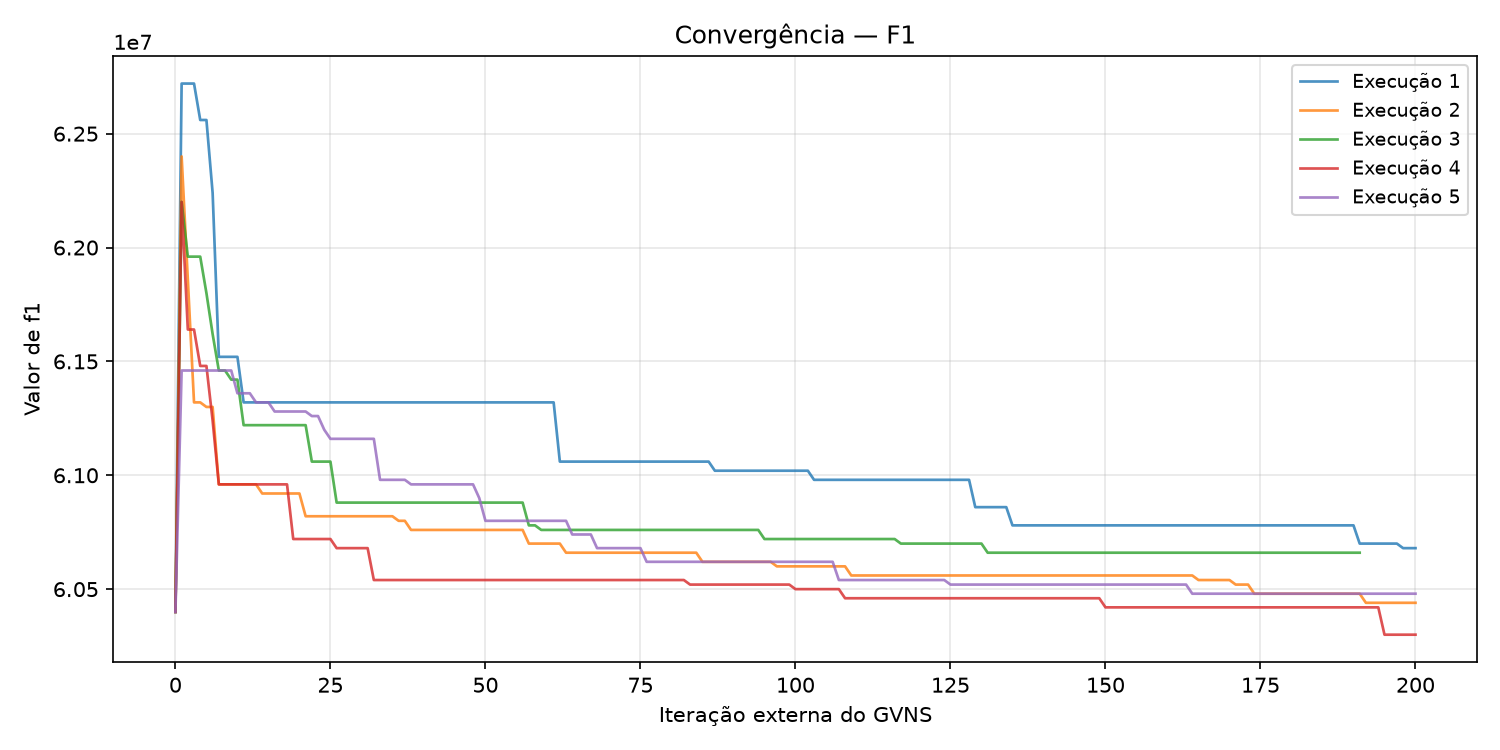
\includegraphics[width=0.9\textwidth]{convergencia_f1.png}
    \caption{Convergência — $f_1$ (custo total de aquisição)}
    \label{fig:conv_f1}
\end{figure}

Para $f_1$, as execuções convergem para valores entre
$60{.}300{.}000$ e $60{.}680{.}000$ R\$. A amplitude entre mínimo e
máximo corresponde a aproximadamente $0{,}63\%$ do menor valor obtido,
indicando baixa dispersão relativa entre as soluções finais. As curvas
também evidenciam que a maior parte das melhorias ocorre nas primeiras
iterações, embora algumas execuções apresentem melhorias adicionais ao
longo da busca.

\begin{figure}[H]
    \centering
    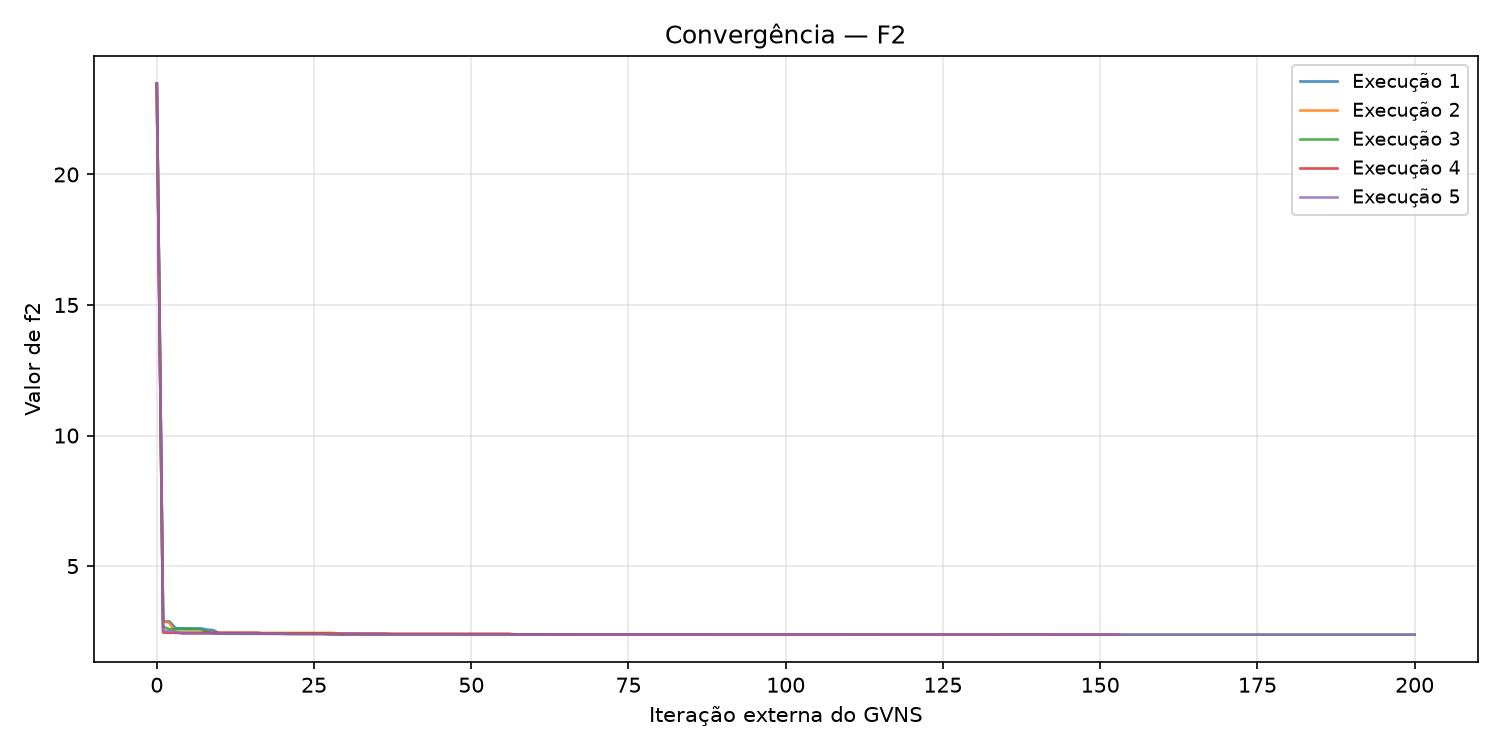
\includegraphics[width=0.9\textwidth]{convergencia_f2.png}
    \caption{Convergência — $f_2$ (desvio quadrático de $SiO_2$)}
    \label{fig:conv_f2}
\end{figure}

Para $f_2$, o valor bruto da função objetivo é reduzido de $23{,}48$
na solução construtiva inicial, que é inviável em qualidade, para cerca
de $2{,}37$ nas melhores soluções finais viáveis, correspondendo a uma
redução aproximada de $90\%$. Essa redução ocorre rapidamente nas
primeiras iterações, e as curvas se estabilizam em valores muito próximos
entre si. O desvio-padrão amostral de $0{,}000543$ representa aproximadamente
$0{,}0229\%$ da média, indicando alta consistência entre as execuções.

\begin{figure}[H]
    \centering
    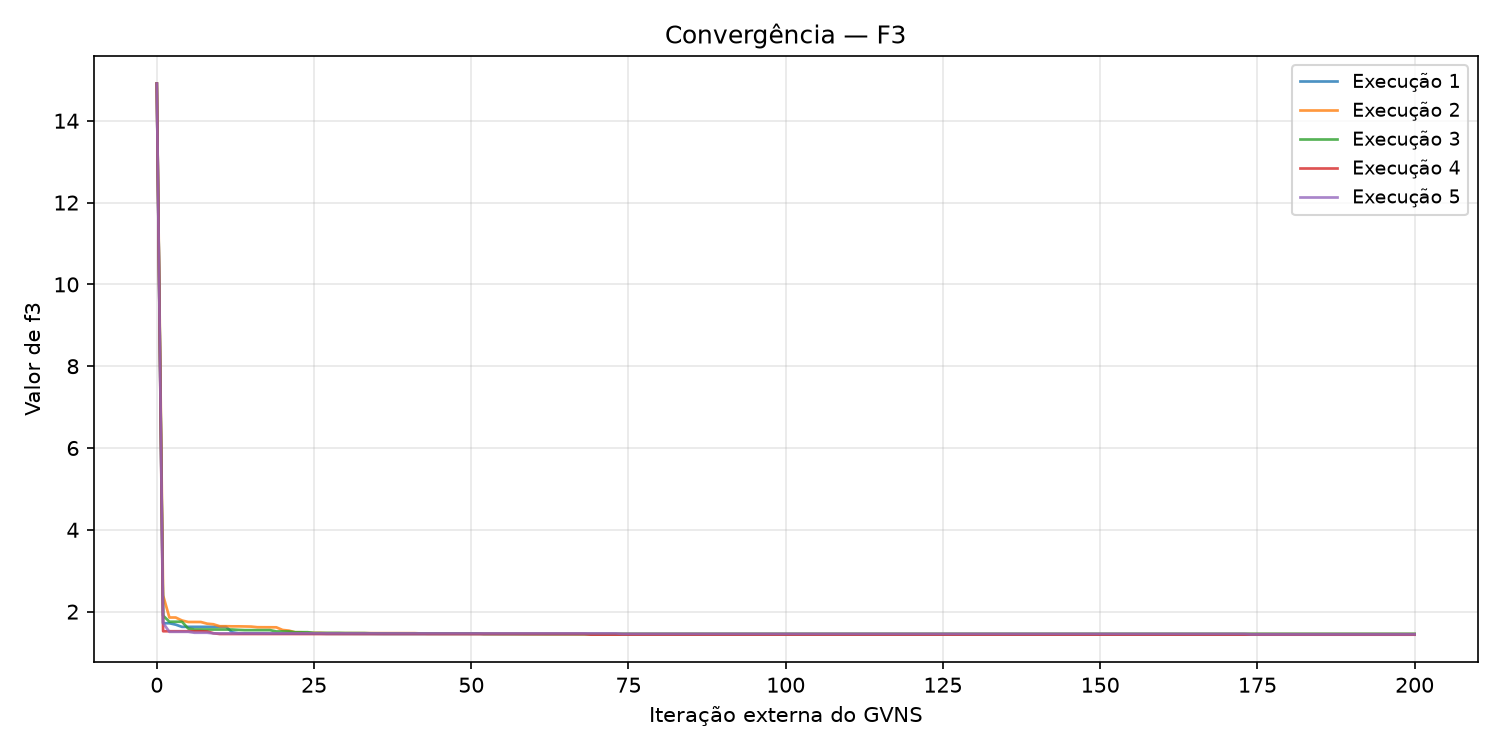
\includegraphics[width=0.9\textwidth]{convergencia_f3.png}
    \caption{Convergência — $f_3$ (desvio quadrático de $Al_2O_3$)}
    \label{fig:conv_f3}
\end{figure}

Para $f_3$, a dinâmica é semelhante à de $f_2$: o valor bruto da função
objetivo passa de $14{,}91$ na solução construtiva inicial, inviável em
qualidade, para aproximadamente $1{,}44$ nas melhores soluções finais
viáveis, também representando redução próxima de $90\%$. A variabilidade
entre execuções é, entretanto, maior: o desvio-padrão é $0{,}007289$
($0{,}50\%$ da média) e a amplitude entre mínimo e máximo é de
aproximadamente $0{,}017$. Essa maior dispersão indica que a busca para
$f_3$ foi mais sensível às escolhas estocásticas realizadas pelo GVNS
nos experimentos conduzidos.


\subsection{Melhor Solução por Objetivo}

As Figuras~\ref{fig:sol_f1}--\ref{fig:sol_f3} apresentam, em barras
empilhadas, a composição da melhor solução encontrada para cada objetivo.
Cada barra representa uma pilha ($P_1$ a $P_{10}$); cada segmento
corresponde a um tipo de minério, e a altura do segmento indica o
número de caminhões de $2$ kt daquele minério alocados à pilha. A altura
total de cada barra é o número total de caminhões da pilha, que varia de
10 ($P_1$, 20 kt) a 19 ($P_{10}$, 38 kt), conforme os dados do problema.

\begin{figure}[H]
    \centering
    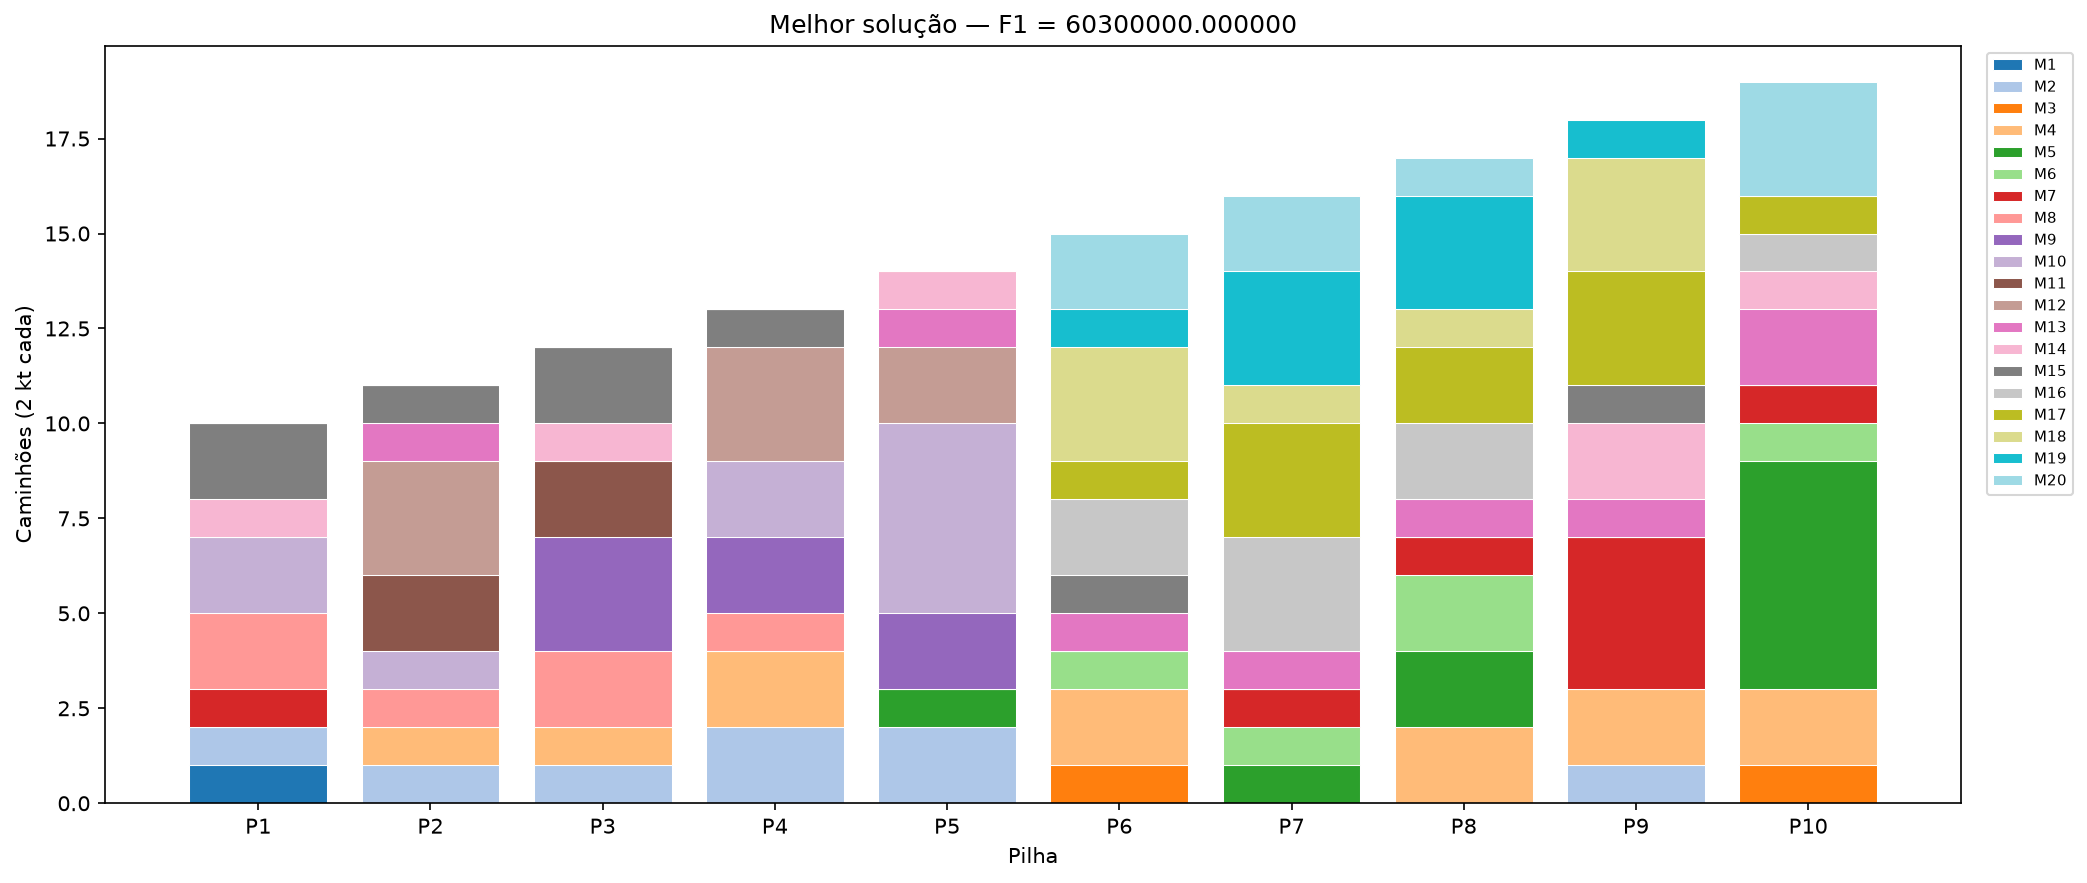
\includegraphics[width=\textwidth]{melhor_solucao_f1.png}
    \caption{Melhor solução — $f_1 = \num{60300000}$ R\$ (seed 789)}
    \label{fig:sol_f1}
\end{figure}

\begin{figure}[H]
    \centering
    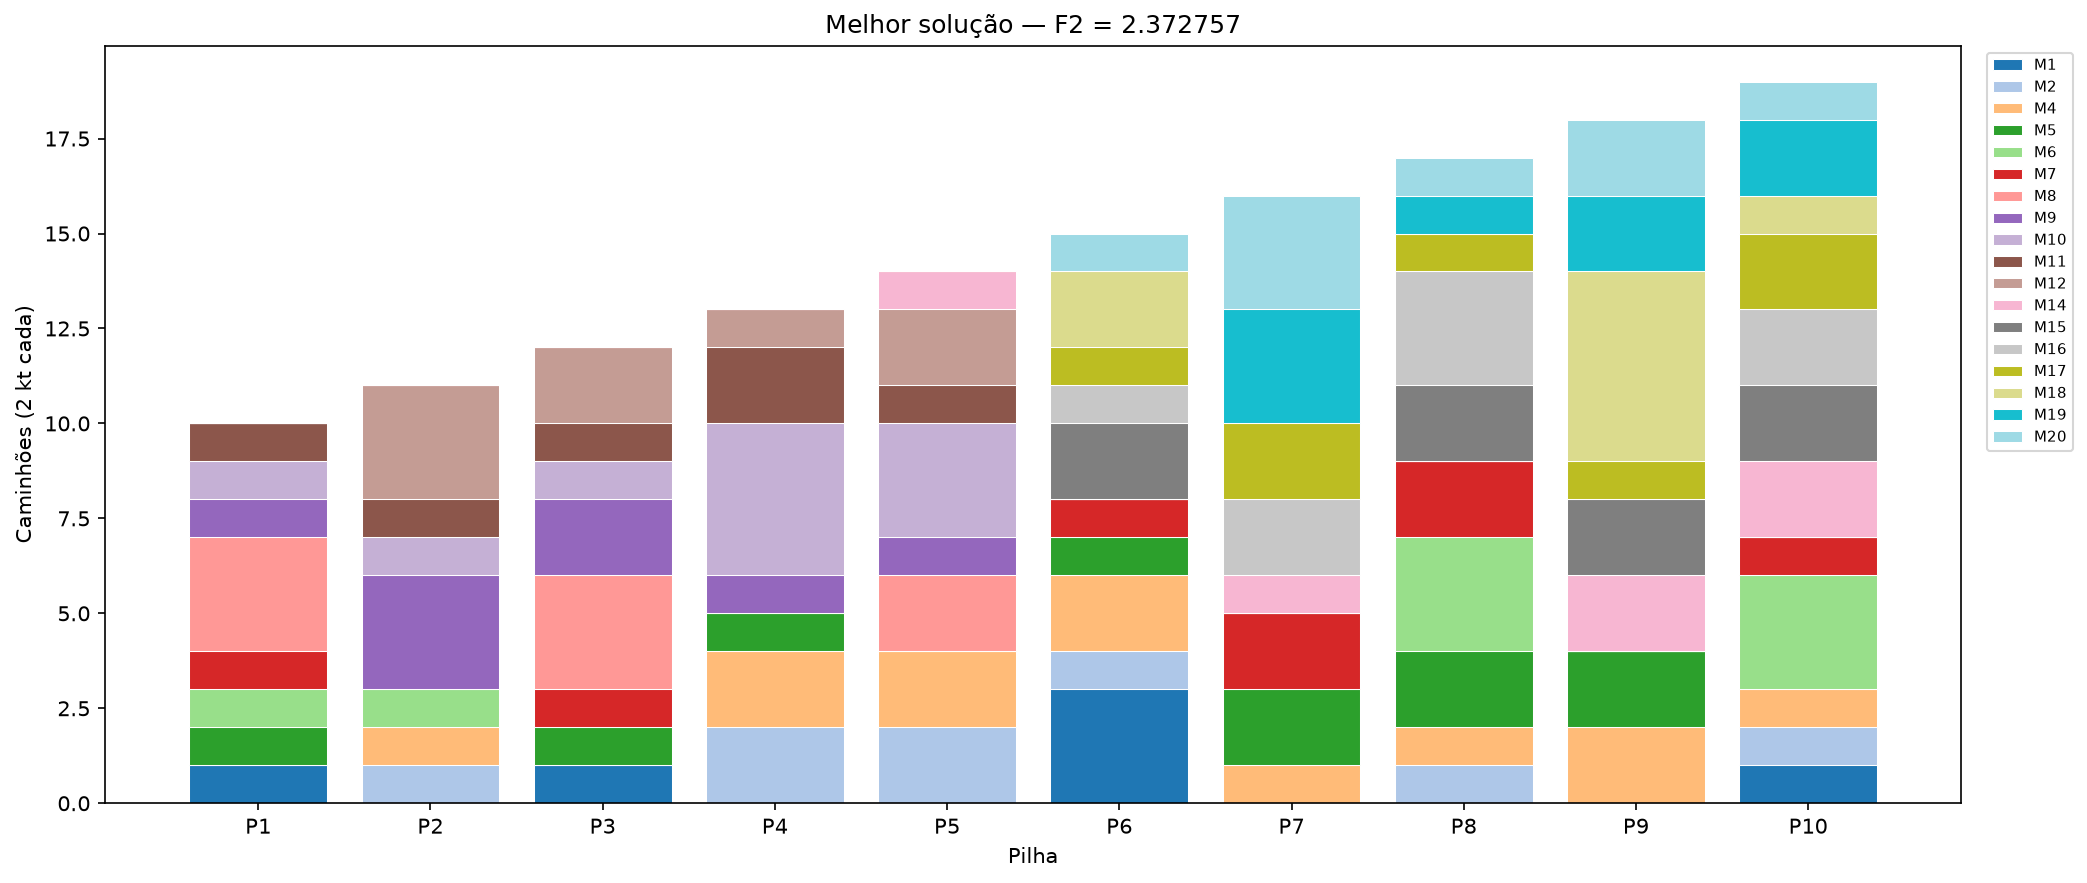
\includegraphics[width=\textwidth]{melhor_solucao_f2.png}
    \caption{Melhor solução — $f_2 = \num{2,372757}$ (seed 456)}
    \label{fig:sol_f2}
\end{figure}

\begin{figure}[H]
    \centering
    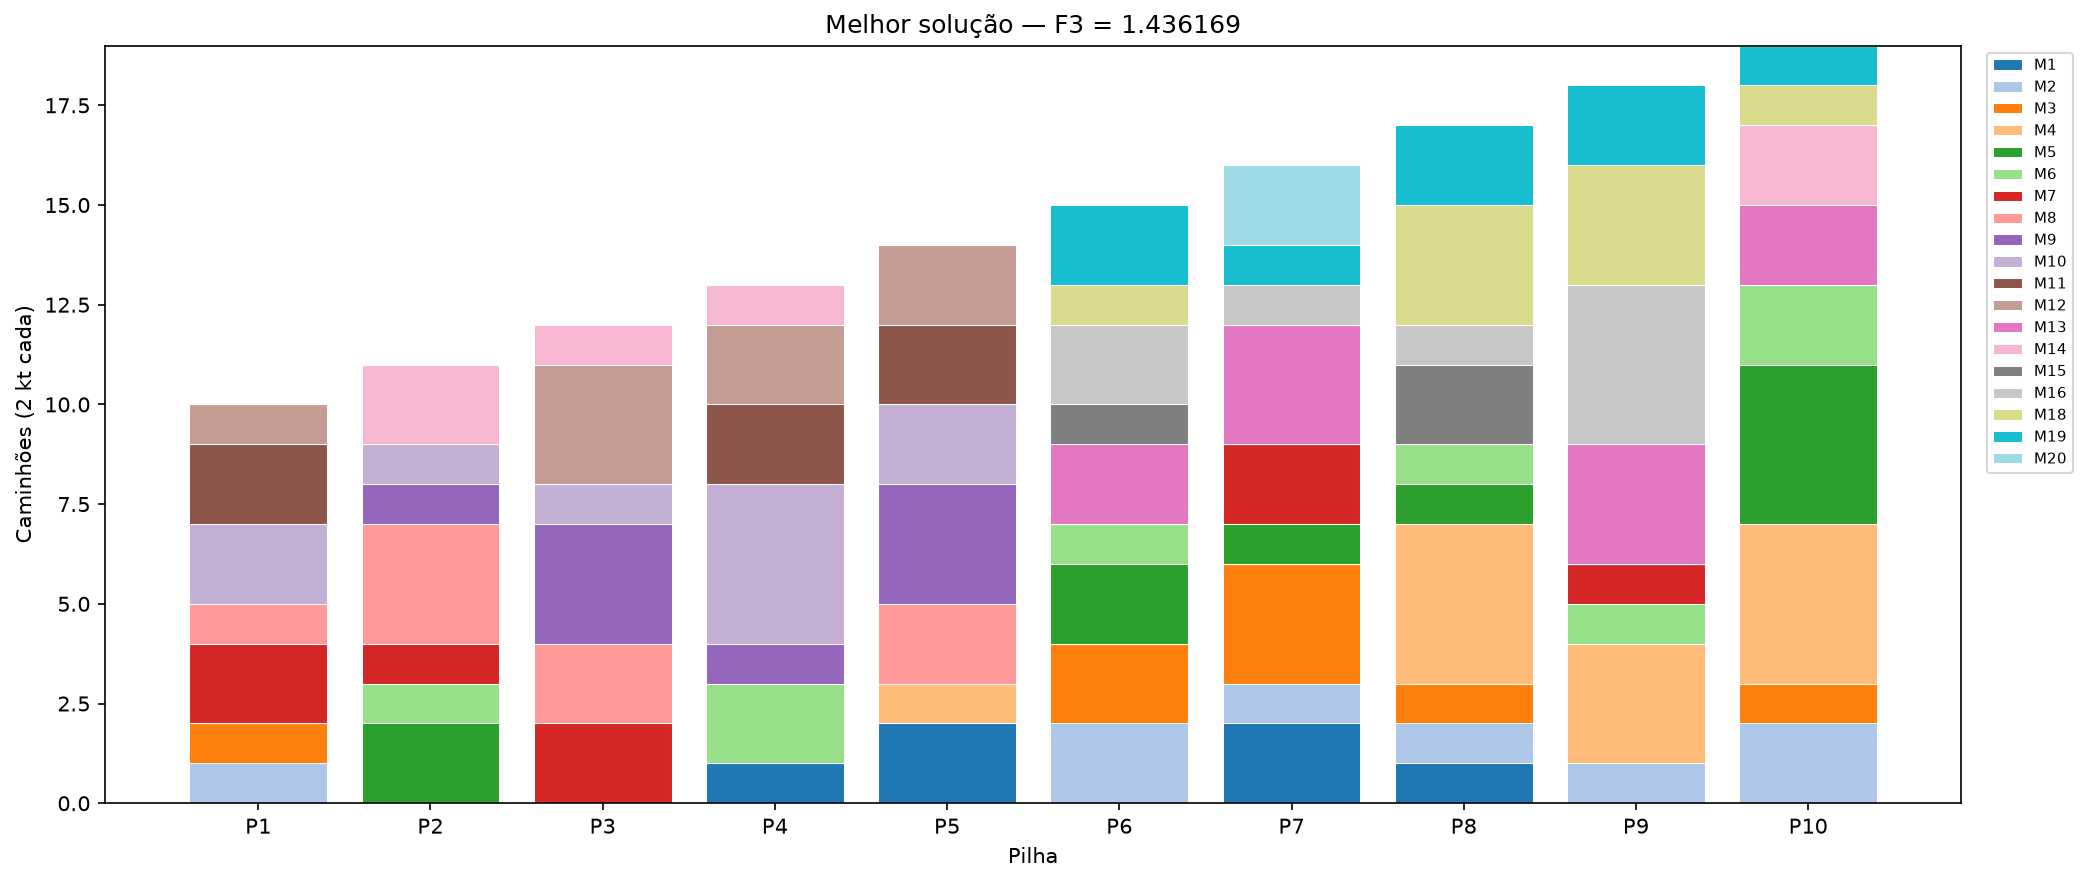
\includegraphics[width=\textwidth]{melhor_solucao_f3.png}
    \caption{Melhor solução — $f_3 = \num{1,436169}$ (seed 789)}
    \label{fig:sol_f3}
\end{figure}

As composições diferem entre os três objetivos, o que era esperado: cada
objetivo prioriza características químicas distintas e, portanto, induz
diferentes combinações de minérios nas pilhas.


\subsection{Análise dos Resultados}

\subsubsection{$f_1$ — Custo total}

A solução construtiva apresenta custo de $60{.}400{.}000$ R\$, porém
viola restrições de qualidade e, portanto, não constitui uma alternativa
final viável. O GVNS encontrou uma solução viável com custo mínimo de
$60{.}300{.}000$ R\$. Assim, além de eliminar as violações de qualidade,
foi possível reduzir em aproximadamente $0{,}17\%$ o custo bruto da
composição inicial. Esse resultado é particularmente relevante porque a
heurística construtiva já prioriza os minérios de menor custo disponíveis,
enquanto o GVNS precisa simultaneamente ajustar a composição para atender
aos limites de $SiO_2$ e $Al_2O_3$.

A variabilidade entre as cinco execuções é pequena: o desvio-padrão de
$159{.}123$ R\$ representa aproximadamente $0{,}26\%$ da média. Isso
indica que, nos experimentos realizados, diferentes sementes conduziram
a soluções finais de custo relativamente próximo, evidenciando baixa
variabilidade do GVNS para esse objetivo.

\subsubsection{$f_2$ — Desvio quadrático de $SiO_2$}

O GVNS reduziu o valor bruto de $f_2$ de $23{,}48$ na solução
construtiva inicial, que é inviável em qualidade, para $2{,}37$ na
melhor solução final viável, uma redução de aproximadamente $90\%$,
concomitante à obtenção de viabilidade. O desvio-padrão amostral de
$0{,}000543$ é o menor entre os três objetivos tanto em valor absoluto
quanto em relação à média ($\approx 0{,}0229\%$). As cinco execuções produziram
resultados muito próximos, indicando alta estabilidade do GVNS para esse
objetivo nas sementes avaliadas.

\subsubsection{$f_3$ — Desvio quadrático de $Al_2O_3$}

Para $f_3$, o valor bruto da função objetivo foi reduzido de $14{,}91$
na solução construtiva inicial, inviável em qualidade, para $1{,}44$ na
melhor solução final viável, também correspondendo a uma redução próxima
de $90\%$ e acompanhada da obtenção de viabilidade. A variabilidade entre
execuções foi maior que em $f_2$: o desvio-padrão foi de $0{,}007289$
($0{,}50\%$ da média) e a amplitude entre mínimo e máximo foi de
aproximadamente $0{,}017$. Essa maior dispersão sugere maior sensibilidade
às escolhas estocásticas do GVNS para $f_3$, embora os experimentos
realizados não permitam caracterizar formalmente a quantidade de ótimos
locais do espaço de busca.

\subsubsection{Comparação entre objetivos}

Todas as execuções produziram soluções finais viáveis quanto à qualidade.
Para $f_2$ e $f_3$, os valores brutos das funções objetivo apresentaram
reduções próximas de $90\%$ em relação à solução construtiva inicial,
que era inviável. Para $f_1$, além de restaurar a viabilidade, o GVNS
obteve pequeno ganho de custo em relação à composição inicial.

Em termos relativos à média, $f_2$ apresentou a menor variabilidade entre
execuções, com desvio-padrão amostral de aproximadamente $0{,}0229\%$. Para $f_1$, o
desvio-padrão correspondeu a aproximadamente $0{,}26\%$ da média,
enquanto $f_3$ apresentou a maior dispersão relativa, de aproximadamente
$0{,}50\%$. Assim, dentre os três experimentos, $f_2$ foi o mais estável
e $f_3$ o mais sensível às diferentes sementes utilizadas.

\section{Conclusão}

Nesta primeira entrega, foram formuladas e resolvidas separadamente as três versões mono-objetivo do problema de formação de pilhas de minério, considerando a minimização do custo total de aquisição, do desvio quadrático de $SiO_2$ e do desvio quadrático de $Al_2O_3$.

A solução foi representada por vetores de caminhões associados às pilhas, e a busca foi realizada por meio de uma metaheurística GVNS composta por três estruturas de vizinhança, perturbação SHAKE e refinamento por VND. As restrições estruturais foram preservadas por construção, enquanto as violações de qualidade foram tratadas por penalização.

Os experimentos realizados em cinco execuções independentes para cada função objetivo mostraram que o método foi capaz de produzir soluções finais viáveis em todos os casos. Para $f_1$, foi obtido custo mínimo de R\$ 60.300.000, com baixa variabilidade entre as execuções. Para $f_2$ e $f_3$, foram observadas reduções próximas de 90\% nos valores brutos das funções objetivo em relação à solução construtiva inicial, acompanhadas da obtenção de viabilidade.

Entre os três objetivos, $f_2$ apresentou a maior estabilidade entre as diferentes sementes, enquanto $f_3$ apresentou maior sensibilidade às escolhas estocásticas do algoritmo. De forma geral, os resultados indicam que a estrutura de GVNS proposta é capaz de explorar adequadamente o espaço de soluções do problema mono-objetivo, conciliando as restrições operacionais com a busca por soluções de melhor qualidade.

Os resultados desta etapa fornecem também a base experimental necessária para as etapas posteriores do projeto, nas quais os diferentes objetivos poderão ser considerados de forma conjunta.

\end{document}
